\documentclass[twocolumn, fontsize=10pt]{article}

\raggedbottom
\setlength{\parskip}{0pt}

\usepackage[margin=0.80in]{geometry}
\usepackage{lipsum,mwe,abstract}
\usepackage[T1]{fontenc}
\usepackage[english]{babel}
\usepackage{fancyhdr}
\pagestyle{fancyplain}
\fancyhead{}
\fancyfoot[C]{\thepage}
\setlength\parindent{0pt}
\usepackage{booktabs,tabularx,caption,hyperref}
\usepackage{natbib}
\usepackage{amsmath,amsfonts,amsthm}
\usepackage{graphicx}
\usepackage{float}
\usepackage{subcaption}
\usepackage{comment}
\usepackage{enumitem}
\usepackage{cuted}
\usepackage{booktabs}
\usepackage{sectsty}
\usepackage{dblfloatfix}
\usepackage{placeins}

\setlength{\dbltextfloatsep}{8pt plus 2pt minus 2pt}
\usepackage{cuted}
\usepackage{capt-of}

\usepackage{graphicx}
\usepackage[dvipsnames]{xcolor}
\renewenvironment{abstract}{
 {\small
  \begin{center}
  \bfseries \abstractname\vspace{-.5em}\vspace{0pt}
  \end{center}
  \list{}{\setlength{\leftmargin}{0mm}\setlength{\rightmargin}{\leftmargin}}
  \item\relax}
 }{\endlist}


\usepackage[]{mdframed}
\makeatletter
\renewcommand{\maketitle}{\bgroup\setlength{\parindent}{0pt}
\begin{flushleft}
  \@title
  \@author \\
  \@date
\end{flushleft}\egroup
}
\makeatother

\newcommand{\framedtext}[1]{%
\par%
\noindent\fbox{%
    \parbox{\dimexpr\linewidth-2\fboxsep-2\fboxrule}{#1}%
}%
}

\definecolor{RBlue}{HTML}{2E4A7C}
\definecolor{RBlueLight}{HTML}{90AEC1}
\definecolor{RSand}{HTML}{F2CB80}
\definecolor{RGray}{HTML}{E0E2DC}
\definecolor{CodeBG}{HTML}{F7F8FA}
\definecolor{ElegantNavy}{HTML}{0E2A47}
\definecolor{SteelBlue}{HTML}{4B6E8A}
\definecolor{DeepGrey}{HTML}{333333}

\usepackage[most]{tcolorbox}
\tcbuselibrary{minted}
\usepackage{minted}

\definecolor{RCharcoal}{HTML}{2B2B2B}

\hypersetup{
  colorlinks=true,
  linkcolor=RBlue,
  citecolor=blue,
  urlcolor=RBlue
}

\colorlet{bg}{CodeBG}
\DeclareTCBListing{mintedbox}{O{}m!O{}}{%
  breakable=true,
  listing engine=minted,
  listing only,
  minted language=#2,
  minted style=default,
  minted options={
    linenos,
    breaklines=true,
    fontsize=\small,
    numbersep=8pt,
    #1},
  boxsep=0pt,
  left=25pt,
  top=3pt,
  bottom=3pt,
  arc=0pt,
  colback=white,
  colframe=SteelBlue,
  boxrule=0pt,
  leftrule=3pt,
  enhanced,
  #3
}

\definecolor{captiongray}{gray}{0.35}
\captionsetup[figure]{font=small, labelfont={bf,color=captiongray}, textfont={color=captiongray}}
\captionsetup[table]{font=small,  labelfont={bf,color=captiongray}, textfont={color=captiongray}}
\captionsetup[subfigure]{font=footnotesize, labelfont={bf,color=captiongray}, textfont={color=captiongray}}

\newtcolorbox{myquote}[1][]{%
    colback=black!5,
    colframe=black!5,
    notitle,
    borderline west={2pt}{0pt}{RoyalBlue!80!black},
    enhanced,
    breakable,
    }

\sectionfont{\color{ElegantNavy}\bfseries\fontsize{11}{13}\selectfont\MakeUppercase}
\subsectionfont{\color{SteelBlue}\bfseries\fontsize{10}{12}\selectfont}
\subsubsectionfont{\color{DeepGrey}\bfseries\fontsize{9}{11}\selectfont}

\title{
\Large
\centering
\textbf{Classifying Cardiac Arrhythmias: A Comparative Analysis} \\
[8pt]
\Large \textcolor{RCharcoal}{Machine Learning, Assignment 3, Time Series Analysis} \\[10pt]}
\date{\today}
\author{{\normalsize Iñigo Arriazu García, Laia Colomé Xicoy, Andrea Pérez Valle, Joana Ros Alonso, Gabriel Torres Zamora}}

\begin{document}
\twocolumn[ \maketitle ]


% ─────────────────────────────────────────────────────────────────────────────
\section{Introduction}
\label{sec:intro}

Cardiac arrhythmias are a leading cause of cardiovascular morbidity worldwide. Reliable automated detection of irregular heartbeats is therefore a clinically important problem \citep{moody2001impact}. Electrocardiogram (ECG) signals encode the electrical activity of the heart as a time series, and individual beats can be classified into clinically meaningful categories by analyzing both their rhythm properties and morphological shape.

This assignment trains, tunes, and compares two sequence-modeling approaches applied to ECG beat classification: a \textit{vanilla Recurrent Neural Network (RNN)} and a \textit{Long Short-Term Memory network (LSTM)}. Both are evaluated on the MIT-BIH Arrhythmia Database \citep{moody2001impact}, one of the most widely used biomedical time-series benchmarks. The primary goal is to classify individual heartbeats into three clinically meaningful categories under the AAMI EC57 standard: Normal (N), Supraventricular ectopic (S), and Ventricular ectopic (V), and to critically compare the two methods.

The two models share a common feature representation: eight features per heartbeat capturing rhythm, morphology, and repolarisation. RNN and LSTM consume these features as a sliding window of $T = 10$ consecutive beats, so each model sees the temporal context of a beat rather than the beat in isolation. Understanding how sequential context interacts with the vanishing gradient problem is a central learning objective of this assignment.


% ─────────────────────────────────────────────────────────────────────────────
\section{Materials and Methods}
\label{sec:methods}

\subsection{Dataset}

The \textit{MIT-BIH Arrhythmia Database} (PhysioNet) is a standard benchmark for ECG beat classification. It contains 48 half-hour excerpts of two-channel ambulatory ECG recordings from 47 subjects, digitised at 360\,Hz with 11-bit resolution. Each beat has been manually annotated by two cardiologists with a symbol indicating its type \citep{moody2001impact}.

We work with the 14-record subset specified in the assignment: records 100, 101, 105, 106, 108, 109, 111, 112, 115, 117, 119, 201, 213, and 219. This subset provides a representative mix of normal sinus rhythm and clinically significant arrhythmias, yielding approximately 30,000 labelled beats after label mapping.

\subsubsection{AAMI 3-Class Scheme}

The raw annotation files contain over 15 distinct beat symbols. Following the AAMI EC57 standard used in most published benchmark results, these are mapped to three classes (Table~\ref{tab:label_map}).

\begin{table}[H]
\centering
\small
\setlength{\tabcolsep}{3pt}
\begin{tabular}{llp{2.8cm}}
\toprule
\textbf{Class} & \textbf{Meaning} & \textbf{Raw symbols} \\
\midrule
N & Normal / bundle branch & \texttt{N . L R e j} \\
S & Supraventricular ectopic & \texttt{A a J S} \\
V & Ventricular ectopic & \texttt{V E} \\
- & Discarded & All other symbols \\
\bottomrule
\end{tabular}
\caption{AAMI 3-class label mapping applied to all 14 records.}
\label{tab:label_map}
\end{table}

Any beat whose symbol does not appear in the mapping (pacemaker beats, noise, rhythm annotations) is discarded. Section~\ref{sec:preprocessing} documents the per-record discard counts.

\subsection{Exploratory Data Analysis}

\subsubsection{ECG Signal Visualisation}

Figure~\ref{fig:ecg_segments} shows 5-second ECG segments for three records with R-peak positions marked and beat types annotated.

% ── FIGURE PLACEHOLDER ──────────────────────────────────────────────────────
% Insert here: task1_ecg_segments.png (or three separate figures for records
% 100, 119, and 201 side by side / stacked).
% Record 100: only N beats, regular rhythm.
% Record 119: mix of N and V beats; V beats arrive earlier and have a
%             different shape and higher amplitude.
% Record 201: all three classes in a single 5-second window; V beats are
%             clearly distinct; S beats are smaller and rounder.
\begin{figure*}[t]
    \centering
    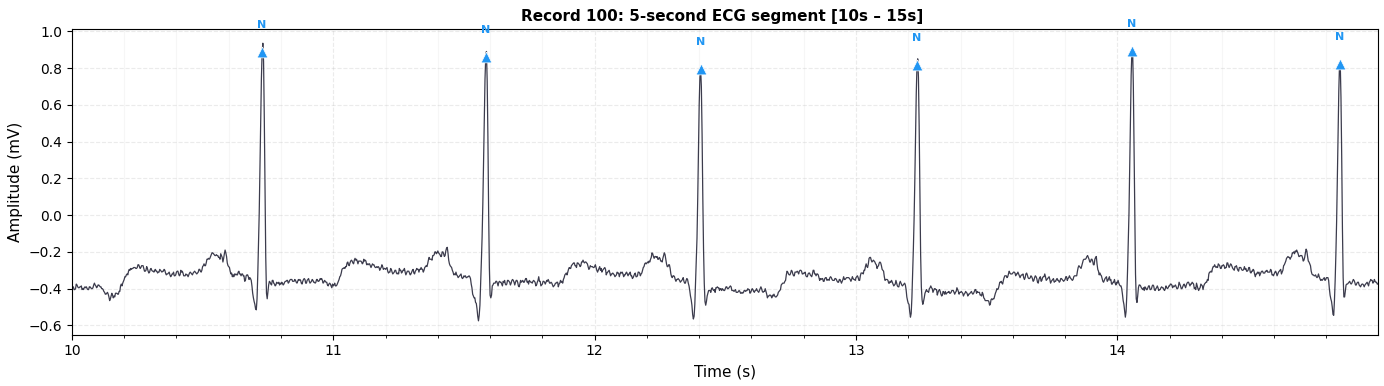
\includegraphics[width=\linewidth]{ecg_!.png}
    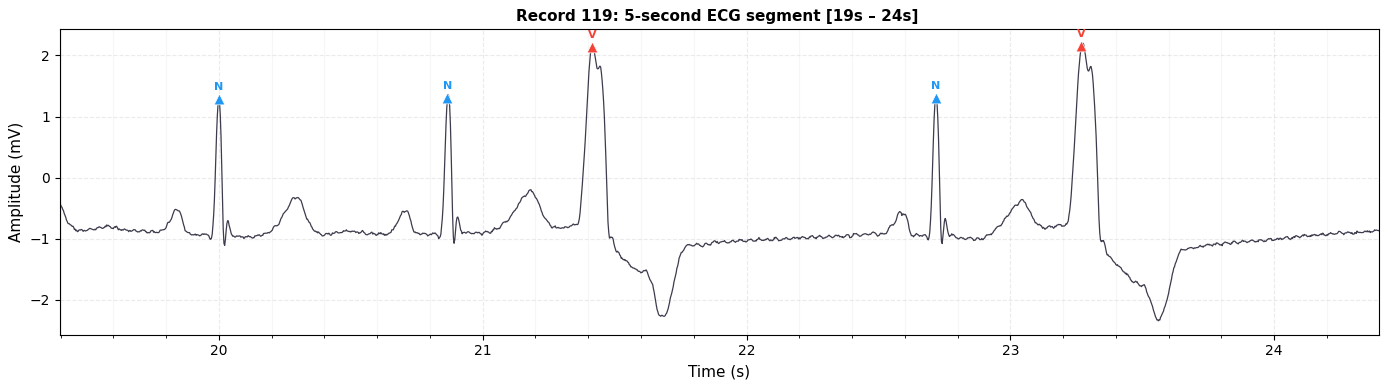
\includegraphics[width=\linewidth]{ecg_2.png}
    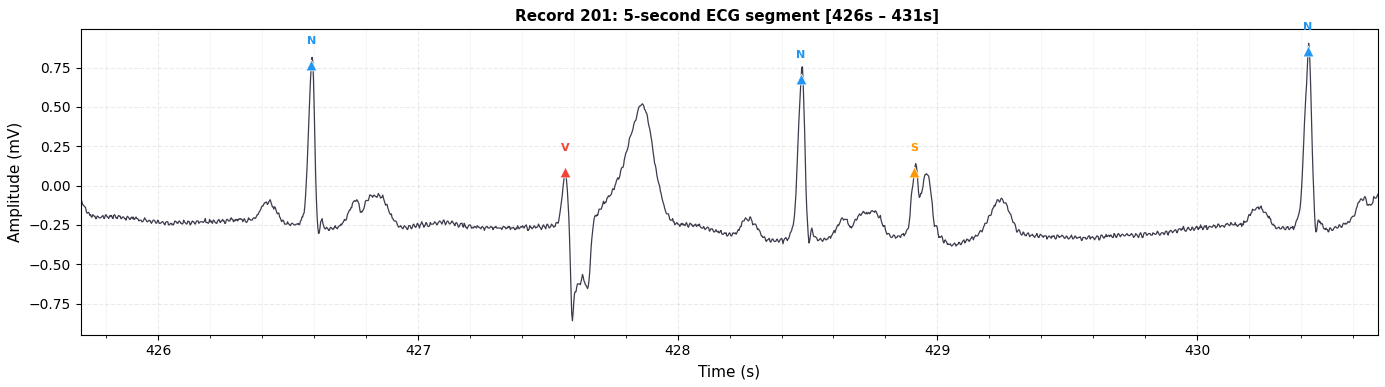
\includegraphics[width=\linewidth]{ecg_3.png}
    \caption{5-second ECG segments (MLII lead) for three MIT-BIH records. Triangular markers indicate R-peak positions coloured by class: blue = N, orange = S, red = V. Record 100 shows only regular N beats; Record 119 shows V beats with distinct shape and earlier arrival; Record 201 contains all three classes within a single 5-second window.}
    \label{fig:ecg_segments}
\end{figure*}
% ────────────────────────────────────────────────────────────────────────────

\subsubsection{Class Distribution}

The dataset is strongly imbalanced: N beats dominate at 94.2\% of all beats, while V accounts for 5.1\% and S for only 0.7\% (Figure~\ref{fig:class_dist}). This imbalance has an important methodological consequence: accuracy alone is insufficient as an evaluation metric. A naive classifier predicting N for every beat would achieve 94.2\% accuracy while failing to detect any arrhythmia. \textbf{Macro F1-score} is therefore used as the primary evaluation metric, as it weights each class equally regardless of frequency.

The imbalance is not uniform across records: records 106 and 119 have notably high V proportions (25.7\% and 22.3\% respectively), and record 201 is the only record with a meaningful number of S beats (6.5\%).

% ── FIGURE PLACEHOLDER ──────────────────────────────────────────────────────
% Insert here: task1_class_distribution.png
% Left panel: bar chart of absolute beat counts per class (N, S, V) across
%             all 14 records combined.
% Right panel: stacked percentage bar chart per record showing class
%              composition.
\begin{figure}[H]
    \centering
    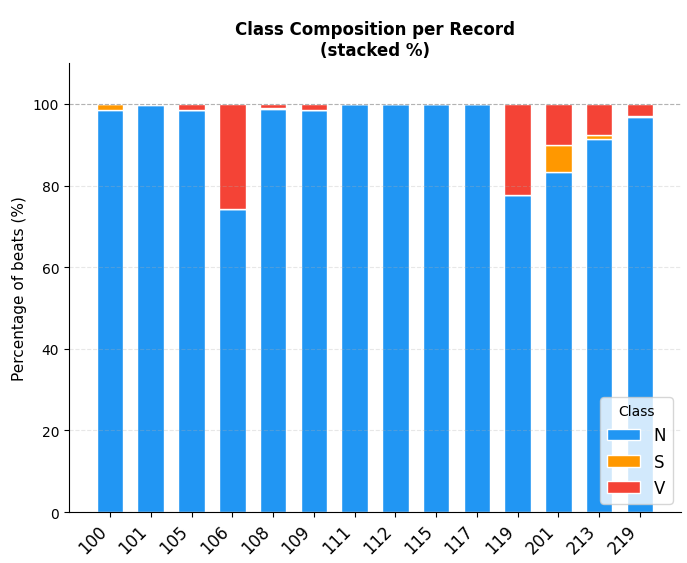
\includegraphics[width=\linewidth]{a3_ml_1.png}
    \caption{Class distribution across 14 MIT-BIH records. Per-record class composition as stacked percentages. N beats dominate (94.2\%); N beats are rare  and V (5.12\%) and there are very few S beats (0.7\%)}
    \label{fig:class_dist}
\end{figure}
% ────────────────────────────────────────────────────────────────────────────


\subsection{Preprocessing and Feature Engineering}
\label{sec:preprocessing}

\subsubsection{Discarded Beats}

A total of 1,057 beats (3.4\% of all annotated beats) were discarded across the 14 records. These fall into six symbol types: fusion beats (\texttt{F}, 369), rhythm-change annotations (\texttt{+}, 252), signal-quality markers (\texttt{\~{}}, 196), non-conducted P-waves (\texttt{x}, 181), isolated QRS artefacts (\texttt{|}, 48), unclassifiable beats (\texttt{Q}, 7), and comment annotations (\texttt{"}, 4). The largest discard counts occur in records 213 (405 beats, mostly \texttt{F}) and 219 (159 beats, mostly \texttt{x}).

\subsubsection{Feature Extraction}

Eight features per beat are engineered from the annotated R-peak positions and the raw signal (Table~\ref{tab:features}). These same features feed every model, making the comparison between RNN and LSTM direct and interpretable. R-peak locations from the \texttt{wfdb} annotation files are used as R-peak positions.

\begin{table}[H]
\centering
\small
\setlength{\tabcolsep}{2pt}
\begin{tabular}{clp{3.2cm}}
\toprule
\textbf{\#} & \textbf{Feature} & \textbf{Clinical meaning} \\
\midrule
1 & \texttt{RR\_current}   & Current RR interval (ms) \\
2 & \texttt{RR\_prev}      & Previous RR interval (ms) \\
3 & \texttt{RR\_ratio}     & RR\_current / RR\_local\_mean \\
4 & \texttt{RR\_local\_mean} & 5-beat rolling mean RR (ms) \\
5 & \texttt{R\_amplitude}  & Signal amplitude at R-peak \\
6 & \texttt{QRS\_duration} & Width of QRS above 50\% of R amplitude (samples) \\
7 & \texttt{QRS\_energy}   & $\sum x^2$ in $\pm$20-sample window \\
8 & \texttt{ST\_mean}      & Mean signal +40 to +120 samples after R-peak \\
\bottomrule
\end{tabular}
\caption{The eight engineered features per beat. Features 1-4 capture rhythm; features 5-8 capture morphology and repolarisation.}
\label{tab:features}
\end{table}

\paragraph{Edge case.} The first beat in each record has no preceding interval. Following the assignment specification, \texttt{RR\_current}, \texttt{RR\_prev}, and \texttt{RR\_local\_mean} for beat 0 are set to the mean RR of the first five available intervals in that record. For beats 1-3, \texttt{RR\_local\_mean} uses the mean of the available preceding intervals.

The resulting feature matrix has shape $(30{,}162 \times 8)$, one row per kept beat across all 14 records, with no missing values.

\subsubsection{Feature Analysis and Correlation}

The per-class feature means and violin plots (Figure~\ref{fig:violin}) reveal clear discriminative patterns. S and V beats have much shorter \texttt{RR\_current} and lower \texttt{RR\_ratio} than N beats, reflecting their premature arrival (mean \texttt{RR\_current}: S $\approx$ 533\,ms, V $\approx$ 720\,ms, N $\approx$ 854\,ms). V beats stand out morphologically: they have approximately twice the \texttt{QRS\_energy} of N beats and the most negative \texttt{ST\_mean} values on average ($-$0.77\,mV), consistent with their wider and more irregular QRS complexes.

% ── FIGURE PLACEHOLDER ──────────────────────────────────────────────────────
% Insert here: task2_feature_distributions.png
% 2x4 grid of violin plots, one per feature, coloured by class
% (blue=N, orange=S, red=V). Horizontal lines indicate class medians.
\begin{figure*}[t]
    \centering
    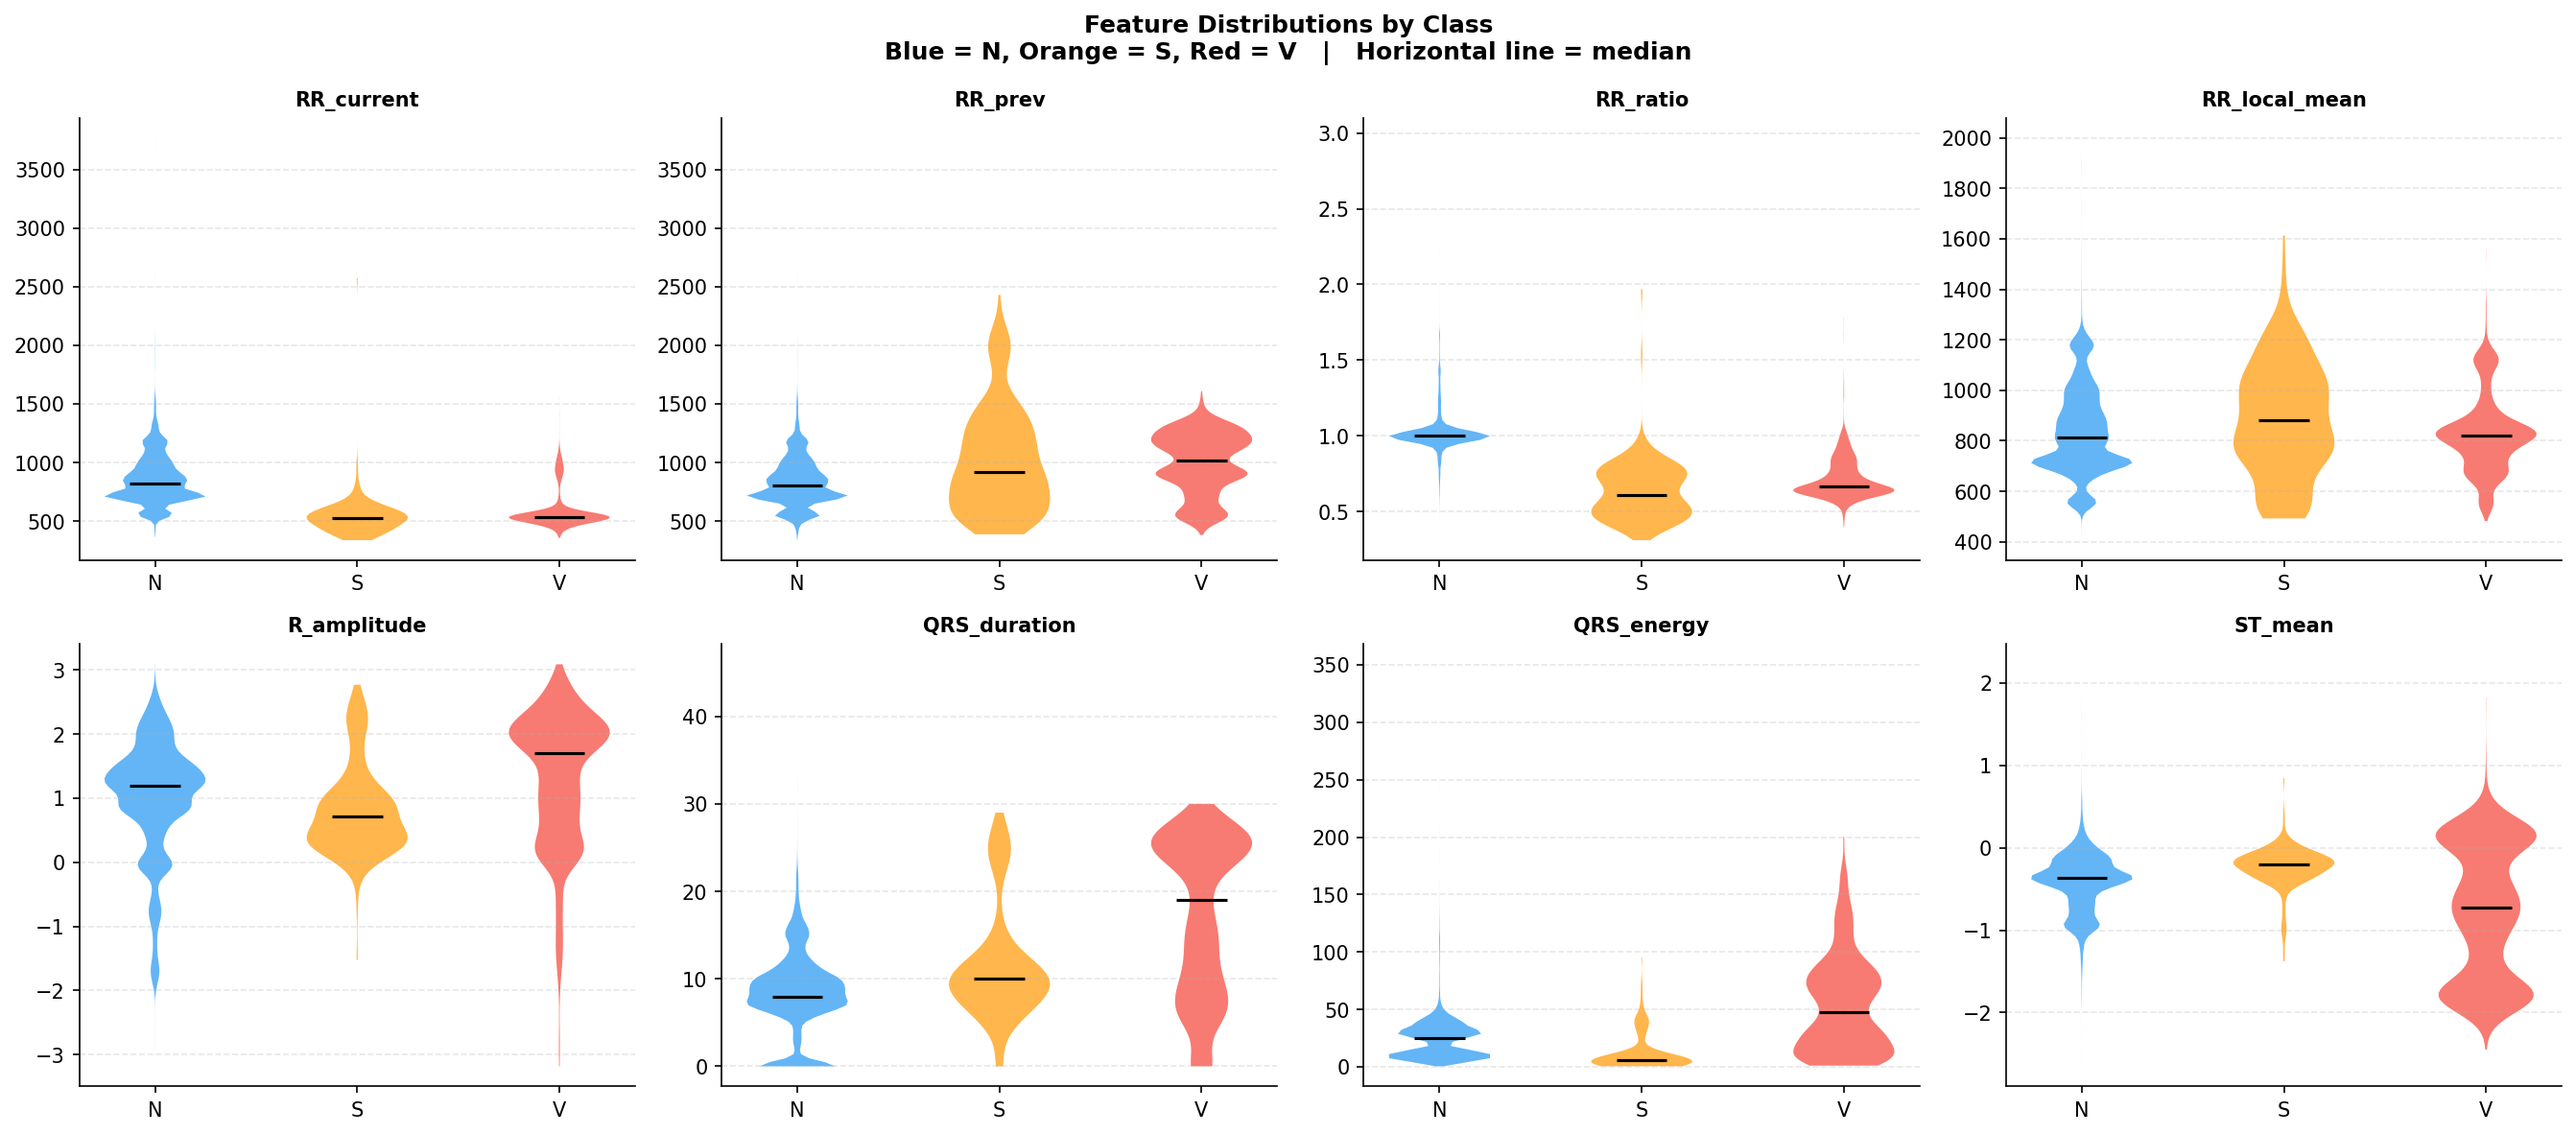
\includegraphics[width=\linewidth]{task2_feature_distributions.png}
    \caption{Feature distributions by class (violin plots). Blue = N, orange = S, red = V. Horizontal lines mark class medians. V beats are most distinguishable via
    \texttt{QRS\_energy} and \texttt{RR\_ratio}; S beats show the shortest \texttt{RR\_current}.}
    \label{fig:violin}
\end{figure*}
% ────────────────────────────────────────────────────────────────────────────

The Pearson correlation heatmap (Figure~\ref{fig:heatmap}) shows that the strongest correlations are among the RR-based features: \texttt{RR\_current} and \texttt{RR\_local\_mean} ($r = 0.81$) and \texttt{RR\_prev} and \texttt{RR\_local\_mean} ($r = 0.78$). This is expected, since \texttt{RR\_local\_mean} is a rolling average that includes the current and previous intervals. \texttt{RR\_ratio} shows near-zero correlation with \texttt{RR\_local\_mean} ($r = 0.03$) and \texttt{R\_amplitude} ($r \approx 0.00$).

% ── FIGURE PLACEHOLDER ──────────────────────────────────────────────────────
% Insert here: task1_correlation_heatmap.png
% 8x8 Pearson correlation heatmap with diverging RdBu_r colourmap.
\begin{figure}[H]
    \centering
    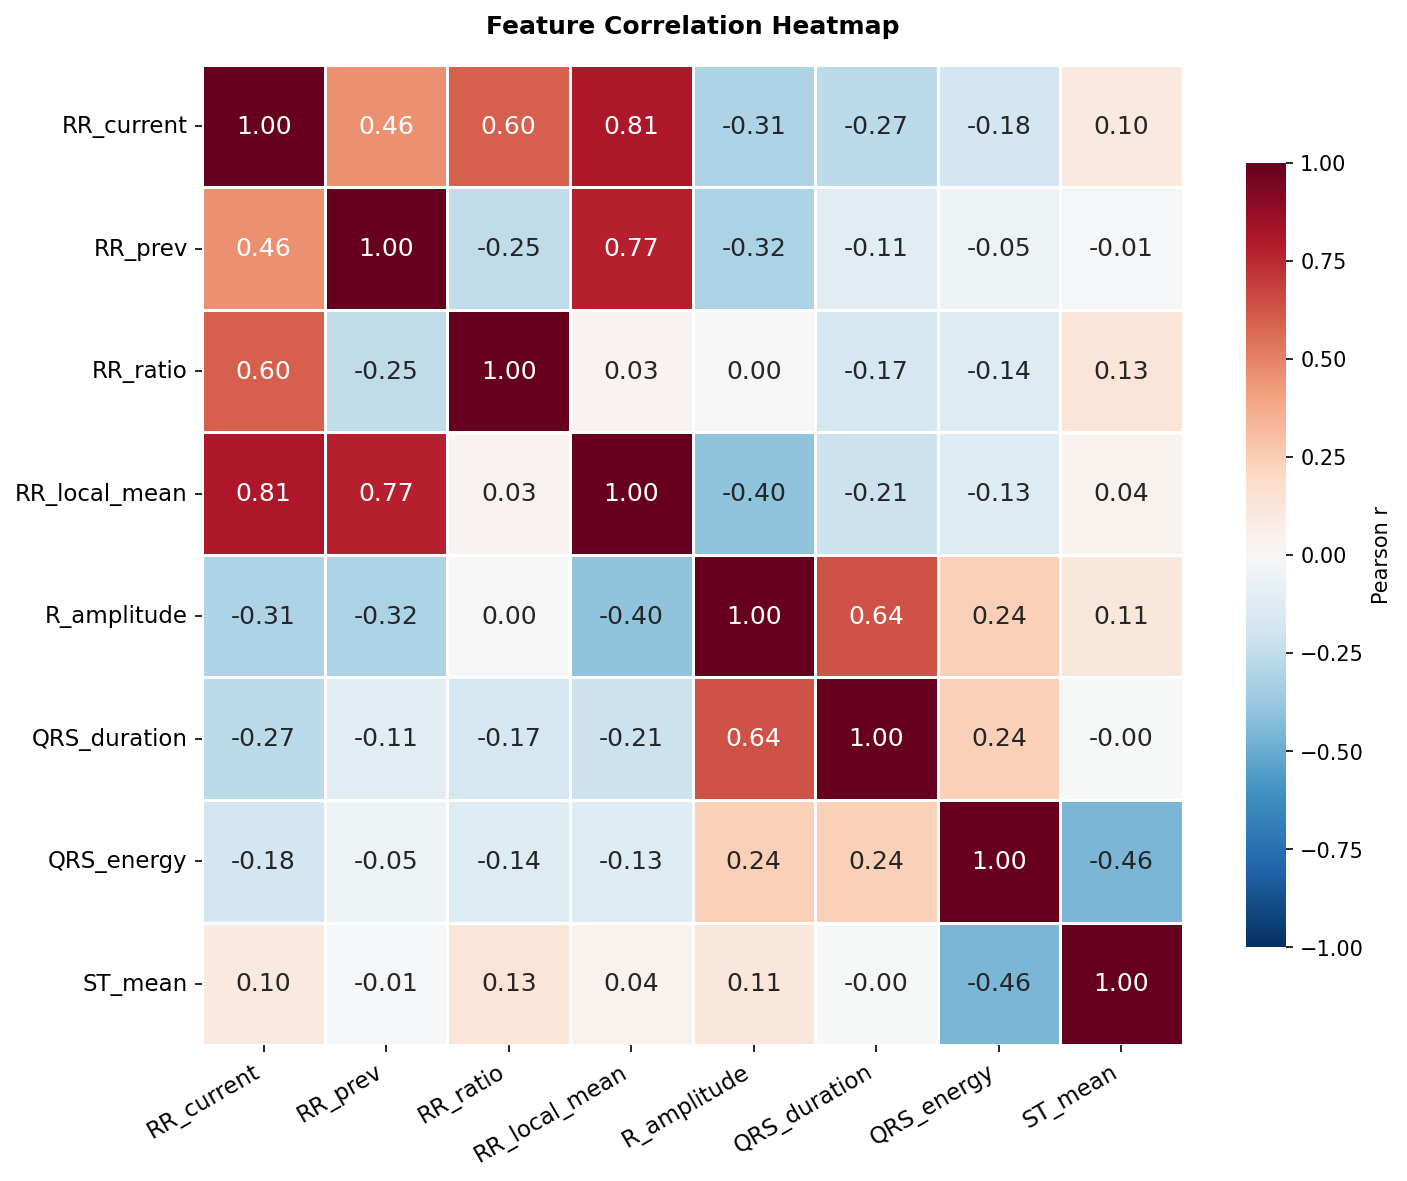
\includegraphics[width=\linewidth]{task1_correlation_heatmap.png}
    \caption{Pearson correlation matrix. Strongest correlations are among RR-based features (RR\_current, RR\_prev, RR\_local\_mean).}
    \label{fig:heatmap}
\end{figure}
% ────────────────────────────────────────────────────────────────────────────

\subsubsection{Temporal Train-Test Split}

Each record is split temporally: beats are sorted by position and the first 80\% go to training ($n = 24{,}124$), the last 20\% to test ($n = 6{,}038$). The cut is applied independently per record. This eliminates window-overlap leakage: with a stride-1 sliding window of $T=10$ beats, two consecutive beats share 9 out of 10 beats in their windows, so a random shuffle would place nearly identical windows in both train and test. A temporal boundary guarantees no window straddles the split. Because the split is not stratified, class proportions differ slightly between splits (Table~\ref{tab:split_balance}).


\begin{table}[H]
\centering
\small
\setlength{\tabcolsep}{3pt}
\begin{tabular}{lrrrr}
\toprule
\textbf{Split} & \textbf{n} & \textbf{N\%} & \textbf{S\%} & \textbf{V\%} \\
\midrule
Full     & 30{,}162 & 94.20 & 0.68 & 5.12 \\
Training & 24{,}124 & 94.40 & 0.62 & 4.98 \\
Test     &  6{,}038 & 93.38 & 0.94 & 5.68 \\
\bottomrule
\end{tabular}
\caption{Class proportions after temporal 80/20 split. Minor differences between splits are expected since the cut is not stratified.}
\label{tab:split_balance}
\end{table}


\subsubsection{Feature Scaling}

\texttt{StandardScaler} is applied to all 8 features, transforming each to zero mean and unit:
\[
    z = \frac{x - \hat{\mu}_{\text{train}}}{\hat{\sigma}_{\text{train}}}
\]

The scaler is \textit{fitted exclusively on the training set} and then applied identically to the test set, preventing any information leakage.

% ── FIGURE PLACEHOLDER ──────────────────────────────────────────────────────
% Insert here: task2_scaling_effect.png
% 2x2 grid: RR_current and R_amplitude before/after StandardScaler.
% Shows that scaling preserves distribution shape but changes axis units.
\begin{figure}[H]
    \centering
    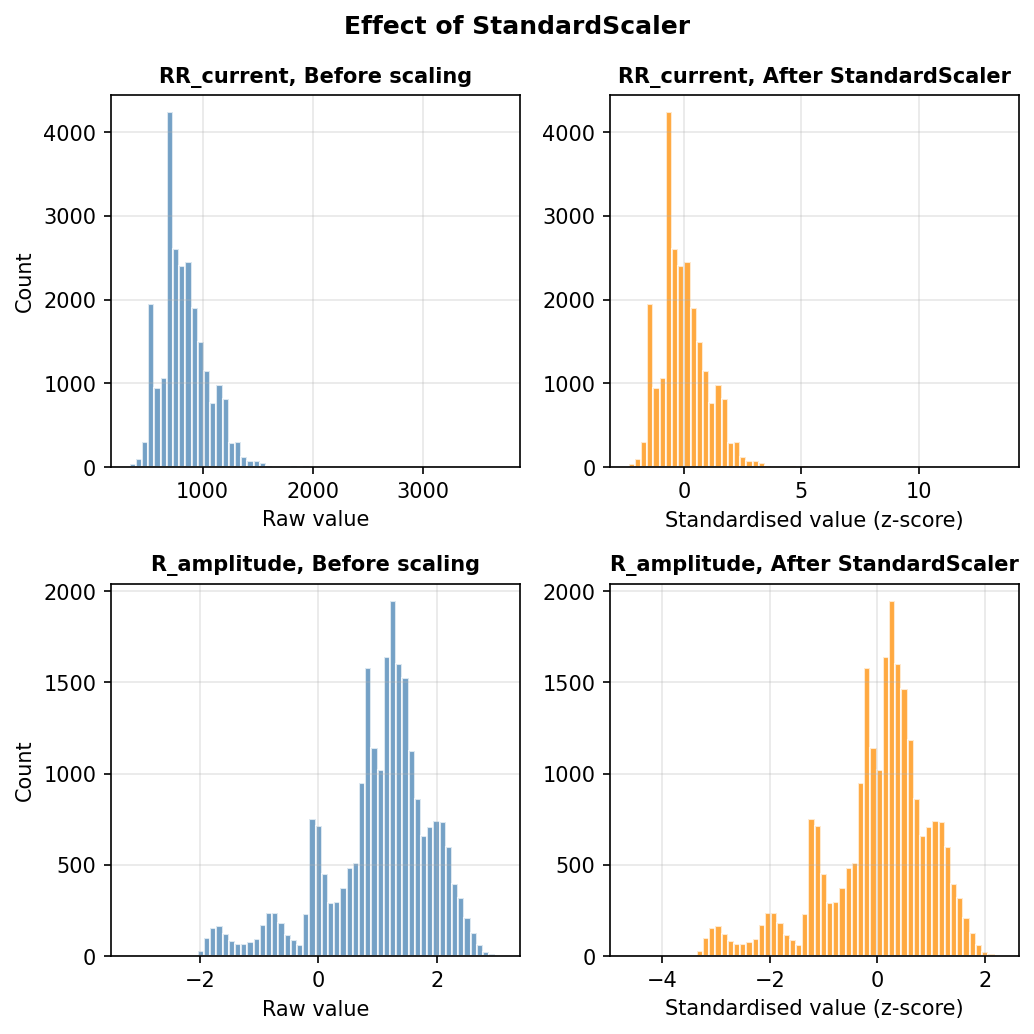
\includegraphics[width=\linewidth]{task2_scaling_effect.png}
    \caption{Effect of StandardScaler on two representative features. Distribution shapes are preserved; only axis units change.}
    \label{fig:scaling}
\end{figure}
% ────────────────────────────────────────────────────────────────────────────

\subsubsection{Sliding Window Dataset}

Since RNN and LSTM are designed to process \textit{sequences} they learn patterns across time.

So, for each beat $i$, we group it together with the 9 beats that came before it, forming a sequence of 10 consecutive beats. This sequence has shape $(10 \times 8)$: 10 beats, each described by 8 features (Figure \ref{fig:windows}). The label assigned to this sequence is the class of beat $i$; the most recent one. As the window slides forward one beat at a time, consecutive windows overlap by 9 beats. The first 9 beats of each record are skipped since they do not have enough history to form a complete window.
Class proportions in the windowed dataset approximately reflect the temporal split, with minor differences due to the $T{-}1$ dropped beats at each record boundary.

% ── FIGURE PLACEHOLDER ──────────────────────────────────────────────────────
% Insert here: task2_window_examples.png
% Three heatmaps (one per class) of shape 8 x 10 showing example windows.
% Each cell is a z-score. Shows V window spike in RR_ratio at beat 9.
\begin{figure*}[t]
    \centering
    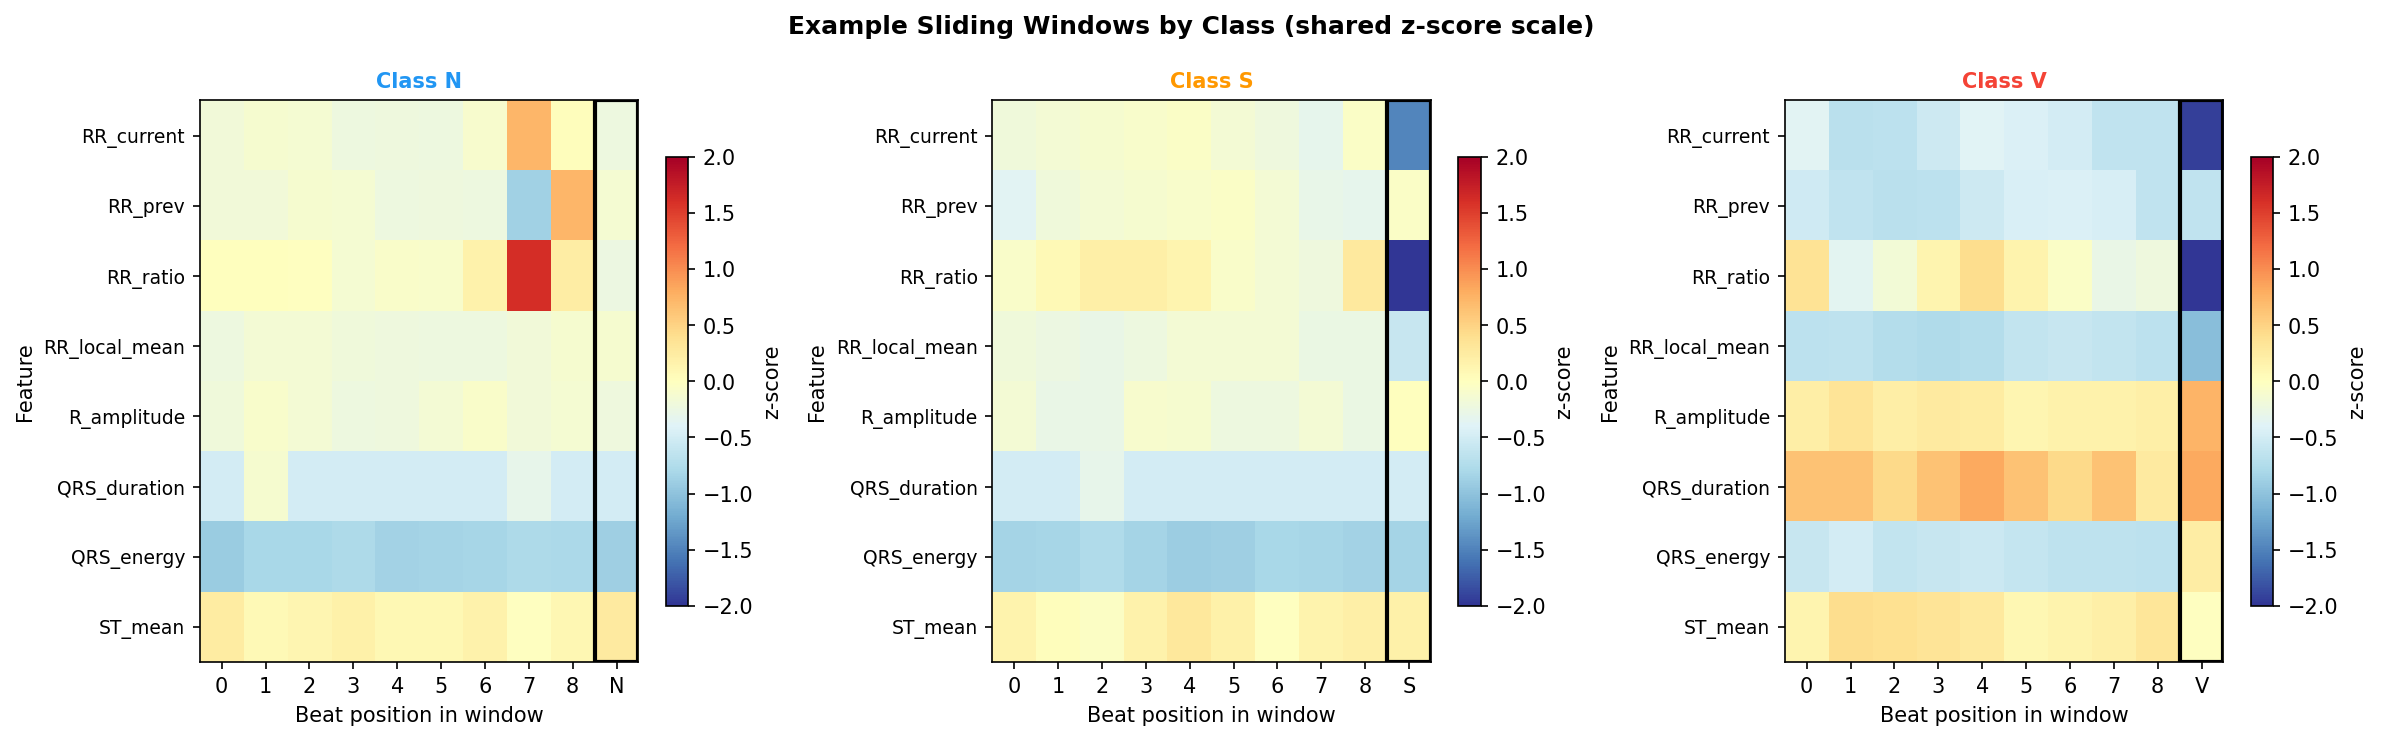
\includegraphics[width=\linewidth]{task2_window_examples.png}
    \caption{Example sliding windows by class (10 beats $\times$ 8 features, z-scores). The V window shows a clear spike in \texttt{RR\_ratio} at beat 9 (current beat arrived much earlier than the local baseline) and a strongly negative \texttt{RR\_prev} (long pause before the ectopic beat). The S window shows a similar but milder pattern. The N window is comparatively uniform across all beat positions.}
    \label{fig:windows}
\end{figure*}
% ────────────────────────────────────────────────────────────────────────────

The PyTorch \texttt{DataLoader} wraps the windowed arrays with \texttt{batch\_size=128} and \texttt{shuffle=True} for training.

% ─────────────────────────────────────────────────────────────────────────────

\section{Classification Methods}
\label{sec:methods_class}

\subsection{Vanilla RNN}

The vanilla RNN classifier is implemented in PyTorch (\texttt{torch.nn.RNN}) with one 
hidden layer of size 64 and a linear output layer mapping the final hidden state to 3 
class scores (logits). The model processes each sliding window of $T=10$ beats 
sequentially, updating a hidden state $h_t \in \mathbb{R}^{64}$ at each step:

\[
h_t = \tanh(W_x x_t + W_h h_{t-1} + b)
\]

where $x_t \in \mathbb{R}^{8}$ is the feature vector for beat $t$, $W_x$ and $W_h$ are 
learned weight matrices, and $b$ is a bias term. Only the final hidden state $h_{10}$ 
is passed to the linear output layer, as it summarises the entire 10-beat context.

Training used cross-entropy loss weighted by inverse class frequency to penalise missed 
S and V beats more heavily than N beats, the Adam optimiser with learning rate 
$\text{lr} = 0.001$, and a fixed seed (\texttt{torch.manual\_seed(42)}) for 
reproducibility. The model was trained for 20 epochs with \texttt{batch\_size} = 128.


\subsubsection{Vanishing Gradient Problem}

The vanilla RNN learns through backpropagation through time (BPTT), which traces 
gradients back through each time step. At each step backwards, the gradient magnitude 
is reduced by repeated multiplication of values smaller than 1 — the derivative of 
$\tanh$ and the weight matrix $W_h$. This causes gradients to shrink exponentially with 
sequence length, effectively giving the model ``amnesia'': the earliest beats in the 
window receive negligible gradient updates and contribute little to learning.

With $T = 10$ beats, the gradient is reduced but remains sufficient for the model to 
learn from all 10 steps. However, for much longer sequences (e.g.\ $T = 100$), the 
gradient signal at the earliest beats would be negligibly small, preventing learning of 
any long-range dependency. This fundamental limitation motivates the use of LSTM, which 
introduces a protected cell state $c_t$ that allows gradients to flow backwards without 
vanishing.

\subsection{LSTM}
The LSTM classifier replaces \texttt{torch.nn.RNN} with \texttt{torch.nn.LSTM},
keeping all other hyperparameters identical (hidden\_size$\,=\,$64,
lr$\,=\,$0.001, 20 epochs, class-weighted cross-entropy, Adam) to ensure a fair
comparison. The only structural difference is that the LSTM maintains both a
hidden state $h_t$ and a \textbf{cell state} $c_t$ governed by three gates:

\begin{align}
f_t &= \sigma(W_f [h_{t-1}, x_t] + b_f) \quad \text{(forget gate)} \nonumber\\
i_t &= \sigma(W_i [h_{t-1}, x_t] + b_i) \quad \text{(input gate)} \nonumber\\
o_t &= \sigma(W_o [h_{t-1}, x_t] + b_o) \quad \text{(output gate)} \nonumber\\
c_t &= f_t \odot c_{t-1} + i_t \odot \tanh(W_c [h_{t-1}, x_t] + b_c) \nonumber\\
h_t &= o_t \odot \tanh(c_t) \nonumber
\end{align}

The cell state $c_t$ provides an additive path for gradients during BPTT,
mitigating the vanishing gradient problem that limits the vanilla RNN on long
sequences. As with the RNN, only the final hidden state $h_{10}$ is passed to
the linear output layer.



% ─────────────────────────────────────────────────────────────────────────────
\section{Results}
\label{sec:results}

\subsection{RNN Training Curves}

Figure~\ref{fig:rnn_curves} shows the training and validation loss and accuracy curves 
for the vanilla RNN over 20 epochs. Both loss curves decrease smoothly and track each 
other closely throughout training, with no sign of overfitting. The gap between training 
accuracy (0.983 at epoch 20) and validation accuracy (0.948) is small and stable.

\begin{figure}[H]
    \centering
    \includegraphics[width=\linewidth]{RNN_loss_curves.png}
    \caption{Training and Validation loss and accuracy curves.}
    \label{fig:rnn_curves}
\end{figure}




\subsection{RNN Classification Performance}

Table~\ref{tab:rnn_report} reports per-class metrics on the test set. The test set 
covers records 106, 119, and 201, which are arrhythmia-rich (records 106 and 119 have 
high V proportions of 25.7\% and 22.3\%; record 201 is the only record with a 
meaningful number of S beats at 6.5\%), making this a harder and more realistic 
evaluation than a random split.

\begin{table}[H]
\centering
\small
\setlength{\tabcolsep}{4pt}
\begin{tabular}{lrrrr}
\toprule
\textbf{Class} & \textbf{Precision} & \textbf{Recall} & \textbf{F1} & \textbf{Support} \\
\midrule
N          & 1.00 & 0.95 & 0.97 & 5{,}526 \\
S          & 0.38 & 0.92 & 0.53 &     51 \\
V          & 0.59 & 0.96 & 0.73 &    335 \\
\midrule
Accuracy   & \multicolumn{3}{r}{0.95} & 5{,}912 \\
Macro F1   & \multicolumn{3}{r}{0.75} & \\
Weighted F1 & \multicolumn{3}{r}{0.96} & \\
\bottomrule
\end{tabular}
\caption{Vanilla RNN classification report on the test set.}
\label{tab:rnn_report}
\end{table}

Figure~\ref{fig:rnn_cm} shows the confusion matrix. The model correctly identifies 
96\% of ventricular beats (only 1 V beat missed out of 335) and 92\% of 
supraventricular beats. The cost of the class-weighted loss is a reduction in N 
precision: 290 N beats are flagged as S or V (false alarms). In a clinical monitoring 
context, false alarms are preferable to missed ventricular beats, which could indicate 
impending cardiac arrest.

\begin{figure}[H]
    \centering
    \includegraphics[width=0.85\linewidth]{RNN_cm.png}
    \caption{Vanilla RNN confusion matrix on the test set. The model 
    misses only 1 V beat out of 335, at the cost of 290 false alarms on N beats.}
    \label{fig:rnn_cm}
\end{figure}

\subsection{LSTM Classification Performance}
The LSTM converges at a similar rate to the RNN (Figure~\ref{fig:lstm_curves}). On the same test set:

\begin{itemize}[nosep]
    \item \textbf{Accuracy}: 0.94
    \item \textbf{Macro F1}: 0.78 \,(+0.04 vs.\ RNN)
    \item \textbf{Weighted F1}: 0.95
\end{itemize}

\begin{table}[H]
\centering
\small
\setlength{\tabcolsep}{4pt}
\begin{tabular}{lrrrr}
\toprule
\textbf{Class} & \textbf{Precision} & \textbf{Recall} & \textbf{F1} & \textbf{Support} \\
\midrule
N          & 1.00 & 0.93 & 0.97 & 5{,}526 \\
S          & 0.64 & 0.84 & 0.73 &     51 \\
V          & 0.49 & 0.99 & 0.65 &    335 \\
\midrule
Accuracy   & \multicolumn{3}{r}{0.94} & 5{,}912 \\
Macro F1   & \multicolumn{3}{r}{0.78} & \\
Weighted F1 & \multicolumn{3}{r}{0.95} & \\
\bottomrule
\end{tabular}
\caption{LSTM classification report on the test set.}
\label{tab:lstm_report}
\end{table}

Compared to the vanilla RNN, the LSTM trades recall for precision on
minority classes. V-beat recall rises from 0.96 to \textbf{0.99} (only
3 missed out of 335), while S-beat precision improves from 0.38 to
\textbf{0.64}, reducing false S alarms. The overall macro F1 improves
from 0.75 to \textbf{0.78}, indicating better-balanced performance
across all three classes. The confusion matrix
(Figure~\ref{fig:lstm_cm}) shows fewer N$\to$S
misclassifications compared to the RNN, at the cost of slightly
lower N recall (0.93 vs.\ 0.95).

\begin{table}[H]
\centering
\small
\setlength{\tabcolsep}{3pt}
\begin{tabular}{lcccccc}
\toprule
\textbf{Model} & \textbf{Acc.} & \textbf{Macro F1} & \textbf{Wt.\ F1} & \textbf{Rec.\,N} & \textbf{Rec.\,S} & \textbf{Rec.\,V} \\
\midrule
Vanilla RNN & 0.95 & 0.75 & 0.96 & 0.95 & 0.92 & 0.96 \\
LSTM        & 0.94 & 0.78 & 0.95 & 0.93 & 0.84 & 0.99 \\
\bottomrule
\end{tabular}
\caption{RNN vs.\ LSTM comparison on the test set.}
\label{tab:rnn_vs_lstm}
\end{table}

% ── FIGURE PLACEHOLDER ──────────────────────────────────────────────────────
\begin{figure}[H]
    \centering
    
\includegraphics[width=\linewidth]{task3_lstm_learning_curves.png}
    \caption{LSTM training and validation curves over 20 epochs.}
    \label{fig:lstm_curves}
\end{figure}

\begin{figure}[H]
    \centering
    
\includegraphics[width=0.85\linewidth]{task3_lstm_confusion_matrix.png}
    \caption{LSTM confusion matrix on the test set.}
    \label{fig:lstm_cm}
\end{figure}
% ────────────────────────────────────────────────────────────────────────────




% ─────────────────────────────────────────────────────────────────────────────

\section{Discussion}
\label{sec:discussion}

\subsection{Effect of Class Imbalance}

The dominance of N beats (94.2\%) means that overall accuracy is a poor proxy for 
model quality on this task. More broadly, this highlights a common pitfall in 
biomedical machine learning: optimising for accuracy on imbalanced datasets can 
produce models that appear strong on paper while being clinically useless. In cardiac monitoring, the consequences of this failure are asymmetric — missing a ventricular 
beat is far more dangerous than a false alarm — which is precisely why evaluation metrics and loss functions must be chosen with the clinical context in mind 
\citep{rajpurkar2017cardiologist}.

\subsection{Sequence Length and the Vanishing Gradient}

The $T = 10$ window is short enough that the vanishing gradient problem does not 
severely limit the vanilla RNN \citep{goodfellow2016deep}. Both models achieve 
comparable overall accuracy ($\sim$0.94--0.95), and the LSTM's macro F1 advantage 
(+0.04) comes primarily from better precision on minority classes rather than from 
exploiting longer-range temporal dependencies. This raises an important question 
about model selection: if the sequence is short enough for a vanilla RNN to learn 
effectively, the added complexity of an LSTM \citep{hochreiter1997lstm} yields only 
marginal gains. The benefit of the LSTM would become more pronounced with longer 
sequences ($T \geq 50$), where the vanilla RNN's gradient signal degrades 
significantly while the LSTM's cell state preserves it.

\subsection{Limitations}

The most significant limitation is the intra-patient split: because beats from the 
same patient appear in both training and test sets, the model is evaluated on rhythm 
patterns it has already partially seen. In a real deployment scenario, a model would 
encounter entirely new patients whose baseline rhythms and arrhythmia patterns differ 
from anything seen during training. A proper inter-patient evaluation is the standard 
approach in published arrhythmia classification benchmarks 
\citep{moody2001impact, rajpurkar2017cardiologist} and would provide a more honest 
estimate of clinical generalisability.


\subsection{RNN vs.\ LSTM Trade-offs}

The two models exhibit a complementary error profile. The vanilla RNN achieves higher
S-beat recall (0.92 vs.\ 0.84) but at the cost of many false S alarms
(precision 0.38). The LSTM reduces these false alarms (S precision 0.64) while
pushing V-beat recall to 0.99, missing only 3 ventricular beats out of 335.
The LSTM's higher macro F1 (0.78 vs.\ 0.75) reflects this more balanced trade-off.

In a clinical context, the choice between the two depends on the monitoring
objective: if maximising detection of any arrhythmia is paramount (minimising
false negatives across S and V), the RNN's higher S recall may be preferred;
if reducing alarm fatigue while maintaining near-perfect V detection is the
priority, the LSTM offers a better balance.

% ─────────────────────────────────────────────────────────────────────────────
\section{Conclusions}
\label{sec:conclusions}

We trained and compared a vanilla RNN and an LSTM on a 3-class ECG beat classification task using the MIT-BIH Arrhythmia Database. Both models were fed identical sliding-window inputs ($T{=}10$ beats $\times$ 8 features) and trained with class-weighted cross-entropy to address the severe class imbalance (94\% N, 5\% V, 1\% S).

The LSTM achieved a higher macro F1 (0.78 vs.\ 0.75) by improving minority-class precision without sacrificing V-beat recall (0.99). However, the modest gap confirms that with $T{=}10$ the vanishing gradient problem does not severely limit the vanilla RNN, and the LSTM's gating mechanism provides only incremental gains at this sequence length.

The main limitation is the intra-patient evaluation protocol: beats from the same patient appear in both splits, so reported metrics overestimate generalisation to unseen patients. Future work should adopt a leave-patient-out split and explore longer sequence lengths where the LSTM's advantage is expected to be more pronounced.



% ─────────────────────────────────────────────────────────────────────────────
\section*{AI Usage}
For this assignment, we used AI tools to help optimise and elaborate our code and improve the overall structure and flow of the text. All core decisions, analytical approaches, and the written report content are our own, based primarily on the class materials and literature.


%─────────────────────────────────────────────────────────────────────────────
\bibliographystyle{plainnat}
\begin{thebibliography}{99}

\bibitem[Moody \& Mark(2001)]{moody2001impact}
Moody, G.~B., \& Mark, R.~G. (2001).
\newblock The impact of the MIT-BIH Arrhythmia Database.
\newblock \textit{IEEE Engineering in Medicine and Biology Magazine}, 20(3), 45--50.

\bibitem[Goldberger et~al.(2000)]{goldberger2000physiobank}
Goldberger, A.~L., et~al. (2000).
\newblock PhysioBank, PhysioToolkit, and PhysioNet: Components of a new research resource for complex physiologic signals.
\newblock \textit{Circulation}, 101(23), e215--e220.

\bibitem[Hochreiter \& Schmidhuber(1997)]{hochreiter1997lstm}
Hochreiter, S., \& Schmidhuber, J. (1997).
\newblock Long short-term memory.
\newblock \textit{Neural Computation}, 9(8), 1735--1780.

\bibitem[Goodfellow et~al.(2016)]{goodfellow2016deep}
Goodfellow, I., Bengio, Y., \& Courville, A. (2016).
\newblock \textit{Deep Learning}.
\newblock MIT Press.

\bibitem[Rajpurkar et~al.(2017)]{rajpurkar2017cardiologist}
Rajpurkar, P., et~al. (2017).
\newblock Cardiologist-level arrhythmia detection with convolutional neural networks.
\newblock \textit{arXiv preprint arXiv:1707.01836}.

\bibitem[Pedregosa et~al.(2011)]{pedregosa2011sklearn}
Pedregosa, F., et~al. (2011).
\newblock Scikit-learn: Machine learning in Python.
\newblock \textit{Journal of Machine Learning Research}, 12, 2825--2830.

\end{thebibliography}

\end{document}